
% ==============================================================
% Introduction
% ==============================================================

\section{Introduction}
\label{sec: Introduction}

In bidirectional traffic, right- and left-hand traffic requires 
vehicles keep either to the right or the left side of the road, 
respectively.\cite{Draper_Geoff_1993} The first right-hand 
traffic law in United State dates back to 1792, applied to the 
Philadelphia and Lancaster Turnpike.
\cite{Weingroff_Richard_2014}\\

The right-hand traffic rule derives regulations on multi-lane 
freeways, which often requires drivers to drive in the 
right-most lane unless they are passing another vehicle, in 
which case they move one lane to the left, pass, and return 
to their former travel lane. The overtaking lane provides 
redundant convenience and safety for vehicles to pass others, 
but lowers freeway's traffic flow capability.\\

Different models may exist that provide a better trade-off 
among traffic flow, safety and convenience. This paper 
considers these three criteria, introduces a different 
freeway traffic model and analyses performances of the two 
models.



% ==============================================================
% Modeling
% ==============================================================

\section{Performance Evaluation}
\label{sec: Performance Evaluation}

Performance of a traffic rule is determined by the three 
criteria below: 

\paragraph{Safety} Average flow density and braking capability 
of vehicles, and lane speed limits, together affect the safety 
state of the freeway. Overtaking action will change local flow 
density and thus disturb the safety state. \textbf{Safety 
factor $\alpha$} is a value that measures how safe a vehicle 
or a lane is, and its value can be calculated from evaluation 
functions discussed at section \ref{sec: Safety Factor}.

\paragraph{Traffic Flow} The usage efficiency of a road is 
called the traffic flow. It can be measured by \textbf{traffic 
flow factor $\beta$}, detailed definition of which is found at 
section \ref{sec: Traffic Flow Factor}.

\paragraph{Convenience} In right- or left-hand traffic, 
overtaking lane is designed redundantly, to provide 
convenience for vehicles in hurry to pass others, or handle 
emergency. Freeways without overtaking lane give extra flow, 
but decrease convenience feature, which is neither described 
in safety nor in traffic flow factors. Hence definition of 
\textbf{convenience factor $\gamma$} is necessary, found at  
section \ref{sec: Convenience Factor}.


\section{Safety Factor}
\label{sec: Safety Factor}

\subsection{Safe Distance Evaluation}
\label{sec: Safe Distance Evaluation}

On the freeway, if a vehicle suddenly slows down, the one 
behind may crash into it. Consequently, a statutory 
distance between each two adjacent vehicles is needed to 
avoid danger. For instance in China, the minimum distance 
is 100 meters between two vehicles on freeway of vehicle 
speed over 100 km/s; and 50 meters on road below 100 km/s.
\cite{PRC_State_Council_Decree_405}\\

We build this model 
to calculate the safe distance between two adjacent cars. 
That is, if the adjacent $d \leq l$ and the car in front 
suddenly slows down,the accident will not happen.\\ \\

\begin{table}
\centering
\begin{tabular}{ll}
\hline
Parameter & Description\\
\hline
$a_1$ & the acceleration of the  car in behind \\
$v_1$ & the velocity of the  car in front \\
$a_2$ & the acceleration of the car in front \\
$v_1$ & the velocity of the  car in front \\
$t_r$ & the driver's reaction time \\
$t$ & the total time whole process \\
$l$ & the safe distance \\
$d$ & a constant which is the real distance between the 
car in front and the car in behind.\\
\hline
\end{tabular}
\caption{Model parameter}
\end{table}

\begin{figure}[h]
\small
\centering
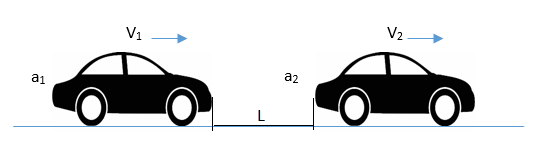
\includegraphics{situation.png}
\caption{}
\end{figure}

There are two possible situations that the accident will 
happen:
\begin{itemize}
\item The accident happens after the car in front stopped.
That is, when
\begin{displaymath}
\frac{v_2}{a_2}  \geq  \frac{v_1}{a_1} + t_r
\end{displaymath}
We have:
\begin{eqnarray}
\frac{v_1^2 - v_0 ^ 2}{2a_1} + v_1 t_r - l & = & \frac{v_2 ^ 2 - v_0 ^ 2}{2a_2}\\
\frac{v_2 - v_0}{a_2} & = & t\\
\frac{v_1 - v_0}{a_1} & = & t - t_r
\end{eqnarray}
\item The collision happens before the car in front stopped. 
That is, when
\begin{displaymath}
\frac{v_2}{a_2}  >  \frac{v_1}{a_1} + t_r
\end{displaymath}
We have:
\begin{eqnarray}
v_1 t_r + \frac{v_1 ^ 2}{2a_1} - l& = &\frac{v_2^2}{2a_2}
\end{eqnarray}
\end{itemize}

Solve this equation array, we have
\begin{displaymath}
l(a_1, a_2, v_1, v_2) = 
\left \{
\begin{array}{cl}
\dfrac{(a_1a_2t_r^2 + 2a_1t_rv_2 + v_1^2 - 2v_1v_2 + v_2^2)}{2(a_1-a_2)} & \dfrac{v_2}{a_2}  \geq \dfrac{v_1}{a_1} + t_r \\
v_2 t_r + \dfrac{v_1 ^ 2}{2a_1} -\dfrac{v_2^2}{2a_2} & \dfrac{v_2}{a_2}  < \dfrac{v_1}{a_1} + t_r
\end{array}
\right .
\end{displaymath}
\\

To calculate $l_{max}$, firstly, we are going to find the extrema,

\begin{displaymath}
\left \{
\begin{array}{cl}
\dfrac{\partial l}{\partial{a_1}} = 0 \\
\dfrac{\partial l}{\partial{a_2}} = 0 \\
\dfrac{\partial l}{\partial{v_1}} = 0 \\
\dfrac{\partial l}{\partial{v_2}} = 0 \\
\end{array}
\right .
\end{displaymath}

This equation array has no solution, which indicates that we can 
get the $l_{max}$ at the boundary of domain.

$l$ reaches the maximum when $a_1$ equals to $a_{min}$, { }$v_1$ 
equals to $v_{1max}$, $v_2$ equals to $v_{2min}$. (If the front 
car drives with the lowest speed, the rear car drives with the 
highest speed, and at the same time, rear car's acceleration is 
the minimum, when emergency happens, the braking distance is 
the longest.)

Thus,
\begin{displaymath}
l_{max}(a_2) = 
\left \{
\begin{array}{cl}
\dfrac{(a_{min}a_2t_r^2 + 2a_{min}t_rv_{min} + v_{max}^2 - 2v_{max}v_{min} + v_{min}^2)}{2(a_{min}-a_2)} & \dfrac{v_{min}}{a_2}  \geq \dfrac{v_1}{a_1} + t_r \\
v_{min} t_r + \dfrac{v_{max} ^ 2}{2a_{min}} -\dfrac{v_{min}^2}{2a_2} & \dfrac{v_2}{a_2}  < \dfrac{v_1}{a_1} + t_r
\end{array}
\right .
\end{displaymath}\\

\paragraph{$l${ } Distribution}
From the result above, we can get $a_2(l)$

%\usepackage{amsmath}
\[ a_2(l) = \begin{cases}
-\dfrac{v_{max}^2 - 2v_{max}v_{min} + 2a_{min}t_rv_{max} + v_{min}^2 - 2a_{min}t_rv_{min} - 2la_{min}}{a_{min}t_r^2 + 2l}, 
\\

\quad l \leq \dfrac{v_{max}^2 - v_{max}v_{min} + 2v_{max}a_{min}t_r - a_{min} v_{min}t_r}{2a_{min}}\\
\dfrac{a_{min}v_{min}^2}{v_{max}^2 + 2a_{min}t_rv_{max} - 2la_{min}}, \quad  l > \dfrac{v_{max}^2 - v_{max}v_{min} + 2v_{max}a_{min}t_r - a_{min} v_{min}t_r}{2a_{min}}
\end{cases}\]
\\

\paragraph{Safety Factor $\alpha$}
For every car, it has a unique safety factor $\alpha$, the 
closer the distance between two adjacent cars is, the smaller 
the $\alpha$ is, vice versa.\\

\begin{figure}[h]
\small
\centering
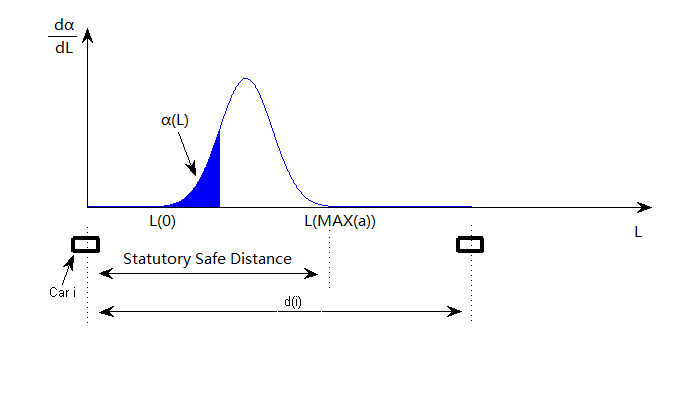
\includegraphics{draw_SafetyNormalDistribution_graph.png}
\caption{safety factor distribution} \label{fig: safety factor distribution}
\end{figure}
\begin{displaymath}
\alpha(l) = \int_{0}^{l} f(x) dx.
\end{displaymath}
%\textbf{Assumptions}\\
%\begin{itemize}
%\item d is the distance between two adjacent cars.
%\end{itemize}
We can see that , when $a_2$ = 0, that is, the front car 
has the lowest deceleration. Since $l(a)$ is a monotone 
increasing function, at this time,$l$ is minimal. In other 
word, it is of little possibility that the distance is less 
than the l, that is, $\alpha(l) \rightarrow 0$                     


\section{Traffic Flow Factor}\label{sec: Traffic Flow Factor}
Since the layout of the cars on the freeway is complicated, 
to simplify, we use a special model to discuss the 
relationship between the safety and traffic flow under the 
situation with and without the right-most rule.
\\
\paragraph{Assumption}

%\begin{itemize}
%\item the rest flow on a single lane drive with a constant speed.

\begin{table}
\centering
\begin{tabular}{ll}
\hline
Parameter & Discription\\
\hline
$k$ & The traffic density\\
$k_j$ & The traffic density under the traffic jam condition\\
$k_m$ & The traffic density when the the traffic flow is the highest.\\
$v_f$ & The velocity when the traffic density is small \\
$Q$ & Traffic flow \\
%$N$ & The total number of the car on the freeway
\hline
\end{tabular}
\caption{Model parameter}
\end{table}

%\subsection{Con Model}
%\paragraph{Assumption}
%\begin{itemize}
%\item Only one car are overtaking, the others are driving with a constant speed
%\item Every overtaking, pass only one car
%\end{itemize}

\begin{equation}
J^* = J_{supply} - J_{need}
\end{equation}

\[ J^* = \begin{cases}
0,\\
\bar{l} - \bar{l}_{max}
\end{cases}\]

%\item Without the right-most rule, there is no overtaking lane, vehicle can stay on either lane at any time.
%\item On the freeway, except the overtaking car, others are subject to the uniform distribution.
%\end{itemize}


\begin{displaymath}
\beta = A\beta_1 + B\beta_2
\end{displaymath}

%\begin{itemize}
%\item 
%\begin{displaymath}
%\beta_1 = \frac{J_1 - J_2}{J_2}
%\end{displaymath}
%\end{itemize}

\begin{table}
\centering
\begin{tabular}{ll}
\hline
Parameter & Meaning\\
\hline
$J$ & traffic flow\\
$J_1$ & the supply traffic flow \\
$J_2$ & the demand traffic flow \\
$s$ & the lenth of a car \\
$l$ & the safe distance \\
$\bar{v}$ & the average velocity\\
\hline
\end{tabular}
\caption{Model parameter}
\end{table}


\section{Convenience Factor}\label{sec: Convenience Factor}


% ==============================================================
% Analysis
% ==============================================================

\section{Model Analysis}


% ==============================================================
% Conclusions
% ==============================================================

\section{Conclusions}



% ==============================================================
% Discussion
% ==============================================================

\section{Discussion}

\subsection{Strengths}
	
\subsection{Weaknesses}



% ==============================================================
% References
% ==============================================================

\begin{thebibliography}{99}

\bibitem{Draper_Geoff_1993} Draper, Geoff (1993). "Harmonised 
Headlamp Design for Worldwide Application". Motor Vehicle 
Lighting. Society of Automotive Engineers. pp. 23-36.

\bibitem{Weingroff_Richard_2014} Weingroff, Richard. "On The 
Right Side of the Road". United States Department of 
Transportation. Retrieved 10 January 2014.

\bibitem{Mick_Hamer_1986} Hamer, Mick. "Left is right on the 
road", New Scientist, 25 December 1986 - 1 January 1987. No.
1540/1541, p.16.

\bibitem{PRC_State_Council_Decree_405} "Regulations for the Implementation of Law of the People's Republic of China on 
Road Traffic Safety". The State Council of the P.R.C., 30 
April 2004. Regulation No.80, Decree No.405.

\end{thebibliography}
